\documentclass[10pt,twocolumn]{article}
%DIF LATEXDIFF DIFFERENCE FILE
%DIF DEL main.tex         Thu May  8 20:53:24 2025
%DIF ADD main_arxiv.tex   Thu May  8 20:55:30 2025
\usepackage[utf8]{inputenc}
%DIF 3c3
%DIF < \usepackage{amsmath,amssymb}
%DIF -------
\usepackage{amsmath} %DIF > 
%DIF -------
\usepackage{graphicx}
\usepackage{xcolor}
\usepackage{tikz}
\usetikzlibrary{petri,positioning}
\usepackage[colorlinks=true,allcolors=blue]{hyperref}
%DIF 9-11d9
%DIF < \usepackage{booktabs}
%DIF < \usepackage{float}
%DIF < \usepackage{enumitem}
%DIF -------

%DIF < % Load custom style file
%DIF -------
\title{\DIFaddbegin \DIFadd{Analysis of Tensorized Petri Nets Using Numerical Reasoning}\DIFaddend } %DIF > 
%DIF < \usepackage{styles/custom}
\author{ %DIF > 
  \DIFaddbegin \DIFadd{Your Name }\\ %DIF > 
  \DIFadd{Department Name }\\ %DIF > 
  \DIFadd{Institution Name }\\ %DIF > 
  \DIFadd{\texttt{email@domain.com} %DIF > 
}\DIFaddend } %DIF > 
\date{\DIFaddbegin \today\DIFaddend } %DIF > 
%DIF PREAMBLE EXTENSION ADDED BY LATEXDIFF
%DIF UNDERLINE PREAMBLE %DIF PREAMBLE
\RequirePackage[normalem]{ulem} %DIF PREAMBLE
\RequirePackage{color}\definecolor{RED}{rgb}{1,0,0}\definecolor{BLUE}{rgb}{0,0,1} %DIF PREAMBLE
\providecommand{\DIFaddtex}[1]{{\protect\color{blue}\uwave{#1}}} %DIF PREAMBLE
\providecommand{\DIFdeltex}[1]{{\protect\color{red}\sout{#1}}} %DIF PREAMBLE
%DIF SAFE PREAMBLE %DIF PREAMBLE
\providecommand{\DIFaddbegin}{} %DIF PREAMBLE
\providecommand{\DIFaddend}{} %DIF PREAMBLE
\providecommand{\DIFdelbegin}{} %DIF PREAMBLE
\providecommand{\DIFdelend}{} %DIF PREAMBLE
\providecommand{\DIFmodbegin}{} %DIF PREAMBLE
\providecommand{\DIFmodend}{} %DIF PREAMBLE
%DIF FLOATSAFE PREAMBLE %DIF PREAMBLE
\providecommand{\DIFaddFL}[1]{\DIFadd{#1}} %DIF PREAMBLE
\providecommand{\DIFdelFL}[1]{\DIFdel{#1}} %DIF PREAMBLE
\providecommand{\DIFaddbeginFL}{} %DIF PREAMBLE
\providecommand{\DIFaddendFL}{} %DIF PREAMBLE
\providecommand{\DIFdelbeginFL}{} %DIF PREAMBLE
\providecommand{\DIFdelendFL}{} %DIF PREAMBLE
%DIF HYPERREF PREAMBLE %DIF PREAMBLE
\providecommand{\DIFadd}[1]{\texorpdfstring{\DIFaddtex{#1}}{#1}} %DIF PREAMBLE
\providecommand{\DIFdel}[1]{\texorpdfstring{\DIFdeltex{#1}}{}} %DIF PREAMBLE
\newcommand{\DIFscaledelfig}{0.5}
%DIF HIGHLIGHTGRAPHICS PREAMBLE %DIF PREAMBLE
\RequirePackage{settobox} %DIF PREAMBLE
\RequirePackage{letltxmacro} %DIF PREAMBLE
\newsavebox{\DIFdelgraphicsbox} %DIF PREAMBLE
\newlength{\DIFdelgraphicswidth} %DIF PREAMBLE
\newlength{\DIFdelgraphicsheight} %DIF PREAMBLE
% store original definition of \includegraphics %DIF PREAMBLE
\LetLtxMacro{\DIFOincludegraphics}{\includegraphics} %DIF PREAMBLE
\newcommand{\DIFaddincludegraphics}[2][]{{\color{blue}\fbox{\DIFOincludegraphics[#1]{#2}}}} %DIF PREAMBLE
\newcommand{\DIFdelincludegraphics}[2][]{% %DIF PREAMBLE
\sbox{\DIFdelgraphicsbox}{\DIFOincludegraphics[#1]{#2}}% %DIF PREAMBLE
\settoboxwidth{\DIFdelgraphicswidth}{\DIFdelgraphicsbox} %DIF PREAMBLE
\settoboxtotalheight{\DIFdelgraphicsheight}{\DIFdelgraphicsbox} %DIF PREAMBLE
\scalebox{\DIFscaledelfig}{% %DIF PREAMBLE
\parbox[b]{\DIFdelgraphicswidth}{\usebox{\DIFdelgraphicsbox}\\[-\baselineskip] \rule{\DIFdelgraphicswidth}{0em}}\llap{\resizebox{\DIFdelgraphicswidth}{\DIFdelgraphicsheight}{% %DIF PREAMBLE
\setlength{\unitlength}{\DIFdelgraphicswidth}% %DIF PREAMBLE
\begin{picture}(1,1)% %DIF PREAMBLE
\thicklines\linethickness{2pt} %DIF PREAMBLE
{\color[rgb]{1,0,0}\put(0,0){\framebox(1,1){}}}% %DIF PREAMBLE
{\color[rgb]{1,0,0}\put(0,0){\line( 1,1){1}}}% %DIF PREAMBLE
{\color[rgb]{1,0,0}\put(0,1){\line(1,-1){1}}}% %DIF PREAMBLE
\end{picture}% %DIF PREAMBLE
}\hspace*{3pt}}} %DIF PREAMBLE
} %DIF PREAMBLE
\LetLtxMacro{\DIFOaddbegin}{\DIFaddbegin} %DIF PREAMBLE
\LetLtxMacro{\DIFOaddend}{\DIFaddend} %DIF PREAMBLE
\LetLtxMacro{\DIFOdelbegin}{\DIFdelbegin} %DIF PREAMBLE
\LetLtxMacro{\DIFOdelend}{\DIFdelend} %DIF PREAMBLE
\DeclareRobustCommand{\DIFaddbegin}{\DIFOaddbegin \let\includegraphics\DIFaddincludegraphics} %DIF PREAMBLE
\DeclareRobustCommand{\DIFaddend}{\DIFOaddend \let\includegraphics\DIFOincludegraphics} %DIF PREAMBLE
\DeclareRobustCommand{\DIFdelbegin}{\DIFOdelbegin \let\includegraphics\DIFdelincludegraphics} %DIF PREAMBLE
\DeclareRobustCommand{\DIFdelend}{\DIFOaddend \let\includegraphics\DIFOincludegraphics} %DIF PREAMBLE
\LetLtxMacro{\DIFOaddbeginFL}{\DIFaddbeginFL} %DIF PREAMBLE
\LetLtxMacro{\DIFOaddendFL}{\DIFaddendFL} %DIF PREAMBLE
\LetLtxMacro{\DIFOdelbeginFL}{\DIFdelbeginFL} %DIF PREAMBLE
\LetLtxMacro{\DIFOdelendFL}{\DIFdelendFL} %DIF PREAMBLE
\DeclareRobustCommand{\DIFaddbeginFL}{\DIFOaddbeginFL \let\includegraphics\DIFaddincludegraphics} %DIF PREAMBLE
\DeclareRobustCommand{\DIFaddendFL}{\DIFOaddendFL \let\includegraphics\DIFOincludegraphics} %DIF PREAMBLE
\DeclareRobustCommand{\DIFdelbeginFL}{\DIFOdelbeginFL \let\includegraphics\DIFdelincludegraphics} %DIF PREAMBLE
\DeclareRobustCommand{\DIFdelendFL}{\DIFOaddendFL \let\includegraphics\DIFOincludegraphics} %DIF PREAMBLE
%DIF AMSMATHULEM PREAMBLE %DIF PREAMBLE
\makeatletter %DIF PREAMBLE
\let\sout@orig\sout %DIF PREAMBLE
\renewcommand{\sout}[1]{\ifmmode\text{\sout@orig{\ensuremath{#1}}}\else\sout@orig{#1}\fi} %DIF PREAMBLE
\makeatother %DIF PREAMBLE
%DIF COLORLISTINGS PREAMBLE %DIF PREAMBLE
\RequirePackage{listings} %DIF PREAMBLE
\RequirePackage{color} %DIF PREAMBLE
\lstdefinelanguage{DIFcode}{ %DIF PREAMBLE
%DIF DIFCODE_UNDERLINE %DIF PREAMBLE
  moredelim=[il][\color{red}\sout]{\%DIF\ <\ }, %DIF PREAMBLE
  moredelim=[il][\color{blue}\uwave]{\%DIF\ >\ } %DIF PREAMBLE
} %DIF PREAMBLE
\lstdefinestyle{DIFverbatimstyle}{ %DIF PREAMBLE
	language=DIFcode, %DIF PREAMBLE
	basicstyle=\ttfamily, %DIF PREAMBLE
	columns=fullflexible, %DIF PREAMBLE
	keepspaces=true %DIF PREAMBLE
} %DIF PREAMBLE
\lstnewenvironment{DIFverbatim}{\lstset{style=DIFverbatimstyle}}{} %DIF PREAMBLE
\lstnewenvironment{DIFverbatim*}{\lstset{style=DIFverbatimstyle,showspaces=true}}{} %DIF PREAMBLE
\lstset{extendedchars=\true,inputencoding=utf8}

%DIF END PREAMBLE EXTENSION ADDED BY LATEXDIFF

\begin{document}
\DIFdelbegin %DIFDELCMD < 

%DIFDELCMD < \title{Analysis of [Your Topic] Using Petri Net Models}
%DIFDELCMD < \author{
%DIFDELCMD <   John Doe\textsuperscript{1} \and Jane Doe\textsuperscript{2} \\
%DIFDELCMD <   \small\textsuperscript{1}University of Example \\
%DIFDELCMD <   \small\textsuperscript{2}Institute of Sample
%DIFDELCMD < }
%DIFDELCMD < \date{\today}
%DIFDELCMD < 

%DIFDELCMD < \author{
  Yohanes Surya\\[2pt]
  \small\textit{AI Toba Project, IT Del}\\[1pt]
  \small\textit{Toba, Indonesia}\\[1pt]
  \small\textit{yohanes.surya@del.ac.id}
}

%DIFDELCMD < 

%DIFDELCMD < %%%
\DIFdelend \maketitle

\DIFdelbegin %DIFDELCMD < \begin{abstract}
%DIFDELCMD < %%%
\DIFdel{This paper presents an analysis of }%DIFDELCMD < [%%%
\DIFdel{specific topic}%DIFDELCMD < ] %%%
\DIFdel{using Petri Net models. We demonstrate how Petri Nets can be effectively used to model and analyze }%DIFDELCMD < [%%%
\DIFdel{specific systems or processes}%DIFDELCMD < ]%%%
\DIFdel{. Our approach combines theoretical foundations with practical applications, providing insights into }%DIFDELCMD < [%%%
\DIFdel{specific findings}%DIFDELCMD < ]%%%
\DIFdel{. The results show that }%DIFDELCMD < [%%%
\DIFdel{brief summary of key results}%DIFDELCMD < ]%%%
\DIFdel{, which has implications for }%DIFDELCMD < [%%%
\DIFdel{specific field or application area}%DIFDELCMD < ]%%%
\DIFdel{.
}%DIFDELCMD < \end{abstract}
%DIFDELCMD < 

%DIFDELCMD < \begin{IEEEkeywords}
%DIFDELCMD < %%%
\DIFdel{Petri Nets, TikZ, formal modeling, concurrent systems, }%DIFDELCMD < [%%%
\DIFdel{other keywords}%DIFDELCMD < ]
%DIFDELCMD < \end{IEEEkeywords}
%DIFDELCMD < 

%DIFDELCMD < %%%
%DIF <  Include sections
\DIFdelend %DIF >  Rest of your existing content from main.tex
The rise of large language models and neural computing has fundamentally transformed how humans reason in partnership with machines, yet this transformation brings new challenges in interpretability, verification, and cognitive alignment. \textbf{What is often overlooked is that these sophisticated AI systems—capable of generating human-like text, solving complex reasoning tasks, and exhibiting seemingly advanced cognition—ultimately operate through nothing more than arithmetic operations at their core.} Every transformer attention mechanism, every matrix multiplication, every embedding lookup fundamentally reduces to addition, multiplication, and their derivatives. This reality underscores a profound insight: even the most complex reasoning and generative processes can be carried out with arithmetic operations alone. The GASing method responds to this fundamental truth by reconceptualizing arithmetic operations through a digit-wise, pattern-recognition framework that serves as a universal computational paradigm—\textbf{anchored in the principle of minimizing its operational vocabulary by grounding all arithmetic in the fundamental operator of addition.}

This approach finds deep resonance with the work of Professor Ron Eglash in Ethno Mathematics, which reveals how diverse cultures have developed sophisticated mathematical concepts through everyday practices and artistic expressions. The fractal patterns found in traditional Indonesian batik (see Situngkir and Surya, 2009), African architecture (see Eglash, 1999), and other indigenous knowledge systems demonstrate how complex mathematical thinking emerges naturally across human cultures. GASing builds upon these insights by formalizing how such pattern-based reasoning can inform modern computational frameworks. In Indonesia, this approach has been successfully scaled through national education initiatives, where GASing's principles have been integrated into the mathematics curriculum, reaching millions of students and demonstrating how culturally-grounded mathematical thinking can enhance computational literacy at scale.

By positioning addition as a meta-operator—capable of expressing the meaning of any symbolic token structure—GASing creates a language-agnostic verification framework that is both interpretable and measurable. This reduction to a core operator allows for direct assessment of computational and cognitive resource consumption, transparent verification of reasoning, and systematic arrangement of operations that parallel both transformer attention mechanisms and human chunking strategies. \textbf{Given that modern LLMs execute billions or even trillions of arithmetic operations during inference alone, any optimization of these fundamental operations—through pattern recognition, lookup mechanisms, or structural rearrangement—would yield substantial improvements in efficiency, regardless of the apparent complexity of the higher-level reasoning being performed.} The result is a unified, cross-referential decision framework in which every logical step is both auditable and adaptable to the cognitive limits of users or the architectural constraints of machines.

The name "GASing" derives from Indonesian terms: Gampang (easy), Asyik (enjoyable), and menyenangkan (interesting), reflecting the method’s dual purpose: making arithmetic accessible for human understanding while providing a rigorous foundation for interpretable AI. Originally developed as a pedagogical tool, GASing now stands as a scalable, mathematically rigorous, and philosophically grounded approach—one that not only mirrors key aspects of modern AI architectures, but also fosters the convergence of human, machine, and organizational reasoning on a shared, minimal, and interpretable operational substrate. This commitment to a common operator is both a practical solution and a necessary condition for the emergence of a unified theory of learning and collaborative intelligence.

\sectionheader{Background and Related Work}
\label{sec:background}

\subsection{Petri Net Fundamentals}

Formally, a Petri Net is a tuple $(P, T, F, M_0)$ where:
\begin{itemize}
    \item $P$ is a finite set of places
    \item $T$ is a finite set of transitions
    \item $F \subseteq (P \times T) \cup (T \times P)$ is a set of arcs
    \item $M_0: P \rightarrow \mathbb{N}$ is the initial marking
\end{itemize}

The dynamics of Petri Nets are governed by the firing of transitions. A transition $t$ is enabled if each input place $p$ has at least as many tokens as the weight of the arc from $p$ to $t$. When a transition fires, it consumes tokens from its input places and produces tokens in its output places according to the weights of the corresponding arcs.

\subsection{Types of Petri Nets}

Several extensions to the basic Petri Net model have been proposed to enhance its modeling power:

\begin{itemize}
    \item \textbf{Colored Petri Nets} \cite{jensen1987coloured}: Extend the basic model by allowing tokens to have data values (colors).
    \item \textbf{Timed Petri Nets}: Incorporate time into the model, allowing for the analysis of temporal properties.
    \item \textbf{Stochastic Petri Nets}: Introduce probabilistic elements to model random behavior.
    \item \textbf{Hierarchical Petri Nets}: Allow for the decomposition of complex models into simpler submodels.
\end{itemize}

\subsection{Applications of Petri Nets}

Petri Nets have been applied to various domains, including:

\begin{itemize}
    \item \textbf{Workflow Management} \cite{van2000workflow}: Modeling and analyzing business processes.
    \item \textbf{Manufacturing Systems}: Modeling production lines and resource allocation.
    \item \textbf{Communication Protocols}: Analyzing the behavior of network protocols.
    \item \textbf{Software Design}: Modeling concurrent and distributed software systems.
\end{itemize}

\subsection{Related Work}

[Include relevant related work here, citing appropriate references from your bibliography]
\section{GASing Implementation and Algorithms}\label{sec:methodology}

\subsection{Addition Algorithm}

The GASing addition algorithm processes numbers from left to right (most significant digit to least significant), contrary to the traditional right-to-left approach. This presents several advantages:

\begin{lstlisting}[language=Python, caption=GASing Addition Algorithm]
function GASing_Addition(a, b):
    result = ""
    carry = 0
    
    # Pad the shorter number with leading zeros
    a = pad_with_zeros(a, len(b))
    b = pad_with_zeros(b, len(a))
    
    # Process from left to right
    for i in range(0, len(a)):
        # Add digits and carry
        digit_sum = int(a[i]) + int(b[i]) + carry
        
        # Determine new digit and carry
        if digit_sum > 9:
            carry = 1
            digit = digit_sum - 10
        else:
            carry = 0
            digit = digit_sum
            
        result += str(digit)
    
    # Add final carry if necessary
    if carry > 0:
        result += str(carry)
        
    return result
\end{lstlisting}

The left-to-right processing allows for:
\begin{itemize}
    \item Earlier termination for approximate calculations
    \item Alignment with human reading order
    \item Potential parallelization in computational contexts
\end{itemize}

\subsection{Multiplication Algorithm}

GASing multiplication extends the addition algorithm through a structured grid approach:

\begin{lstlisting}[language=Python, caption=GASing Multiplication Algorithm]
function GASing_Multiplication(a, b):
    # Initialize result grid
    rows = len(b)
    cols = len(a)
    grid = initialize_grid(rows, cols)
    
    # Fill multiplication grid
    for i in range(rows):
        for j in range(cols):
            grid[i][j] = int(b[i]) * int(a[j])
    
    # Apply carry propagation using pattern recognition
    apply_carries(grid)
    
    # Convert grid to result
    result = grid_to_result(grid)
    
    return result
\end{lstlisting}

The grid-based approach facilitates:
\begin{itemize}
    \item Visualization of the multiplication process
    \item Systematic carry handling
    \item Identification of patterns in partial products
\end{itemize}

\subsection{Subtraction and Division}

Subtraction in GASing employs the complement method, where negative results at any position trigger borrowing operations in a systematic way. Division extends subtraction through iterative processes with optimization for common patterns.

<<<<<<< HEAD
\subsection{Problem Definition}

[Define the specific problem you are addressing with your Petri Net model]

\subsection{Proposed Petri Net Model}

Our proposed Petri Net model for [specific system or process] consists of the following components:

\begin{itemize}
    \item \textbf{Places}: Represent [specific states or conditions in your system]
    \item \textbf{Transitions}: Represent [specific events or actions in your system]
    \item \textbf{Tokens}: Represent [specific resources or entities in your system]
\end{itemize}

\begin{figure}[htbp]
\centering
\begin{tikzpicture}[scale=0.75, every node/.style={font=\small,transform shape}, node distance=1.2cm]
  % Places
  \placewithtokens{p1}{0,0}{2}        % Resource
  \placewithtokens{p2}{6,0}{0}        % Process
  \placewithtokens{p3}{3,-2.5}{1}     % Control
  \placewithtokens{p4}{9,-2.5}{0}     % Output
  \placewithtokens{p5}{3,-5.5}{0}     % Complete

  % Transitions
  \node[transition] (t1) at (3,0) {};    % Start
  \node[transition] (t2) at (6,-2.5) {}; % Execute
  \node[transition] (t3) at (1,-4) {};   % Cancel
  \node[transition] (t4) at (5,-4) {};   % Finish

  % Arcs
  \draw[pre] (p1) -- (t1);
  \draw[post] (t1) -- (p2);
  \draw[pre] (p3) -- (t1);
  \draw[post] (t1) -- (p3);

  \draw[pre] (p2) -- (t2);
  \draw[pre] (p3) -- (t2);
  \draw[post] (t2) -- (p4);

  \draw[pre] (p3) -- (t3);
  \draw[post] (t3) -- (p5);

  \draw[pre] (p4) -- (t4);
  \draw[post] (t4) -- (p5);

  % Labels for places
  \node[above] at (p1.north) {Resource};
  \node[above] at (p2.north) {Process};
  \node[left] at (p3.west) {Control};
  \node[above] at (p4.north) {Output};
  \node[below] at (p5.south) {Complete};

  % Labels for transitions
  \node[above] at (t1.north) {Start};
  \node[above] at (t2.north) {Execute};
  \node[left] at (t3.west) {Cancel};
  \node[right] at (t4.east) {Finish};

  % Title
  \node[above=1cm] at (3,0) {Petri Net Model of a Simple Workflow Process};
\end{tikzpicture}
\caption{Generic Petri Net model structure for [specific system or process]}
\label{fig:petri_net_generic_model}
\end{figure}

To illustrate common concurrency problems that can be modeled with Petri Nets, we present the Dining Philosophers problem (Figure \ref{fig:dining_philosophers}) and the Producer-Consumer problem (Figure \ref{fig:producer_consumer_workflow}).

\begin{figure*}[htbp]
\centering
% Petri Net Model of the Dining Philosophers Problem (Refined)
\begin{tikzpicture}[node distance=2.2cm and 2.2cm, >=stealth, bend angle=30, auto, on grid]
    % Philosopher thinking states
    \placewithtokens{p1}{0,0}{1}
    \placewithtokens{p2}{3,0}{1}
    \placewithtokens{p3}{1.5,-2.6}{1}

    % Philosopher eating states
    \placewithtokens{e1}{-1.2,-1.5}{0}
    \placewithtokens{e2}{4.2,-1.5}{0}
    \placewithtokens{e3}{1.5,-4.1}{0}

    % Forks
    \placewithtokens{f1}{0,-1.5}{1}
    \placewithtokens{f2}{3,-1.5}{1}
    \placewithtokens{f3}{1.5,-1.5}{1}

    % Transitions (pick up forks)
    \node[transition, rounded corners=2pt] (t1) [below left=0.7cm and 0.7cm of p1] {};
    \node[transition, rounded corners=2pt] (t2) [below right=0.7cm and 0.7cm of p2] {};
    \node[transition, rounded corners=2pt] (t3) [below=0.7cm of p3] {};

    % Transitions (put down forks)
    \node[transition, rounded corners=2pt] (r1) [left=1.2cm of e1] {};
    \node[transition, rounded corners=2pt] (r2) [right=1.2cm of e2] {};
    \node[transition, rounded corners=2pt] (r3) [below=1.2cm of e3] {};

    % Arcs for Philosopher 1
    \draw[pre] (p1) -- (t1);
    \draw[pre] (f1) -- (t1);
    \draw[pre] (f3) -- (t1);
    \draw[post] (t1) -- (e1);
    \draw[pre] (e1) -- (r1);
    \draw[post] (r1) -- (p1);
    \draw[post] (r1) -- (f1);
    \draw[post] (r1) -- (f3);

    % Arcs for Philosopher 2
    \draw[pre] (p2) -- (t2);
    \draw[pre] (f2) -- (t2);
    \draw[pre] (f3) -- (t2);
    \draw[post] (t2) -- (e2);
    \draw[pre] (e2) -- (r2);
    \draw[post] (r2) -- (p2);
    \draw[post] (r2) -- (f2);
    \draw[post] (r2) -- (f3);

    % Arcs for Philosopher 3
    \draw[pre] (p3) -- (t3);
    \draw[pre] (f1) -- (t3);
    \draw[pre] (f2) -- (t3);
    \draw[post] (t3) -- (e3);
    \draw[pre] (e3) -- (r3);
    \draw[post] (r3) -- (p3);
    \draw[post] (r3) -- (f1);
    \draw[post] (r3) -- (f2);

    % Labels for philosophers
    \node[above] at (p1.north) {P1 thinking};
    \node[above] at (p2.north) {P2 thinking};
    \node[below] at (p3.south) {P3 thinking};
    \node[left] at (e1.west) {P1 eating};
    \node[right] at (e2.east) {P2 eating};
    \node[below] at (e3.south) {P3 eating};

    % Labels for forks
    \node[below left] at (f1.south west) {Fork 1};
    \node[below right] at (f2.south east) {Fork 2};
    \node[above] at (f3.north) {Fork 3};

    % Title
    \node[above=1cm] at (current bounding box.north) {Petri Net Model of the Dining Philosophers Problem};
\end{tikzpicture}
\caption{Petri Net model of the Dining Philosophers problem}
\label{fig:dining_philosophers}
\end{figure*}

% First instance of linear_petri_net as a resized figure
\begin{figure}[htbp]
\centering
\resizebox{0.88\columnwidth}{!}{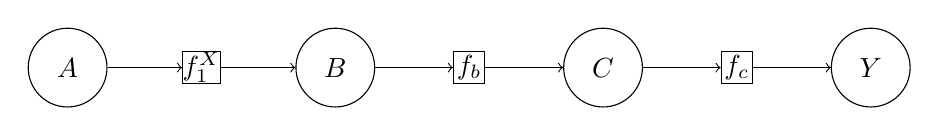
\begin{tikzpicture}[every place/.style={minimum size=10mm}, node distance=1.7cm]
  % Places
  \node[place] (A) {$A$};
  \node[transition] (fa) [right of=A] {$f_1^X$};
  \node[place] (B) [right of=fa] {$B$};
  \node[transition] (fb) [right of=B] {$f_b$};
  \node[place] (C) [right of=fb] {$C$};
  \node[transition] (fc) [right of=C] {$f_c$};
  \node[place] (Y) [right of=fc] {$Y$};

  % Arcs
  \draw[->] (A) -- (fa);
  \draw[->] (fa) -- (B);
  \draw[->] (B) -- (fb);
  \draw[->] (fb) -- (C);
  \draw[->] (C) -- (fc);
  \draw[->] (fc) -- (Y);
\end{tikzpicture}}
\caption{Resized Linear Petri Net}
\label{fig:linear_petri_resized}
\end{figure}

% Second instance as a regular figure
\begin{figure}[htbp]
\centering
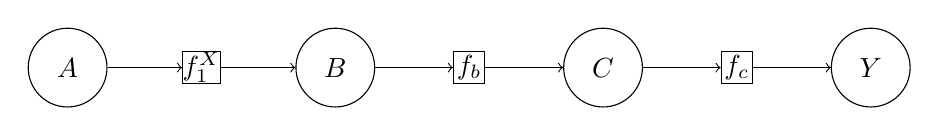
\begin{tikzpicture}[every place/.style={minimum size=10mm}, node distance=1.7cm]
  % Places
  \node[place] (A) {$A$};
  \node[transition] (fa) [right of=A] {$f_1^X$};
  \node[place] (B) [right of=fa] {$B$};
  \node[transition] (fb) [right of=B] {$f_b$};
  \node[place] (C) [right of=fb] {$C$};
  \node[transition] (fc) [right of=C] {$f_c$};
  \node[place] (Y) [right of=fc] {$Y$};

  % Arcs
  \draw[->] (A) -- (fa);
  \draw[->] (fa) -- (B);
  \draw[->] (B) -- (fb);
  \draw[->] (fb) -- (C);
  \draw[->] (C) -- (fc);
  \draw[->] (fc) -- (Y);
\end{tikzpicture}
\caption{Tensorized Petri Net Structure}
\label{fig:tensor_petri}
\end{figure}

\begin{figure}[htbp]
% Petri Net Model of the Producer-Consumer Problem (Refined)
\begin{tikzpicture}[node distance=2.2cm and 2.2cm, >=stealth, bend angle=30, auto, on grid]
    % Places
    \placewithtokens{producer}{-0.5,0}{1}
    \placewithtokens{buffer}{3.3,0}{0}
    \placewithtokens{consumer}{6.5,0}{1}
    \placewithtokens{bufferCapacity}{2.8,-2.2}{3}

    % Transitions
    \node[transition, rounded corners=2pt] (produce) [right=of producer] {};
    \node[transition, rounded corners=2pt] (consume) [right=1.8cm of buffer] {};

    % Arcs
    \draw[pre] (producer) -- (produce);
    \draw[post] (produce) -- (producer);
    \draw[post] (produce) -- (buffer);
    \draw[pre] (buffer) -- (consume);
    \draw[pre] (consumer) -- (consume);
    \draw[post] (consume) -- (consumer);
    \draw[pre] (bufferCapacity) -- (produce);
    \draw[post] (consume) -- (bufferCapacity);

    % Labels
    \node[above=6pt] at (producer.north) {Producer};
    \node[above=14pt] at (buffer.north) {Buffer};
    \node[above=6pt] at (consumer.north) {Consumer};
    \node[below] at (bufferCapacity.south) {Buffer Capacity};
    \node[above] at (produce.north) {Produce};
    \node[above] at (consume.north) {Consume};

    % Title
    \node[above=1cm] at (current bounding box.north) {Petri Net Model of the Producer-Consumer Problem};
\end{tikzpicture}
\caption{Producer-Consumer Workflow}
\label{fig:producer_consumer_workflow}
\end{figure}

\begin{figure}[htbp]
\centering
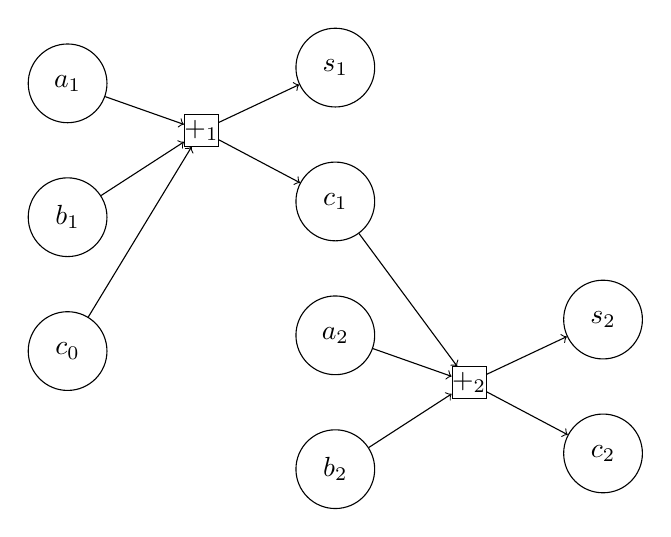
\begin{tikzpicture}[every place/.style={minimum size=10mm}, node distance=1.7cm and 2.2cm]
  % First digit addition
  \node[place] (a1) {$a_1$};
  \node[place, below of=a1] (b1) {$b_1$};
  \node[place, below of=b1] (c0) {$c_0$};
  \node[transition] (add1) [right of=b1, yshift=1.1cm] {$+_1$};
  \node[place] (s1) [right of=add1, yshift=0.8cm] {$s_1$};
  \node[place] (c1) [below of=s1] {$c_1$};

  \draw[->] (a1) -- (add1);
  \draw[->] (b1) -- (add1);
  \draw[->] (c0) -- (add1);
  \draw[->] (add1) -- (s1);
  \draw[->] (add1) -- (c1);

  % Second digit addition
  \node[place, below of=c1] (a2) {$a_2$};
  \node[place, below of=a2] (b2) {$b_2$};
  \node[transition] (add2) [right of=b2, yshift=1.1cm] {$+_2$};
  \node[place] (s2) [right of=add2, yshift=0.8cm] {$s_2$};
  \node[place] (c2) [below of=s2] {$c_2$};

  \draw[->] (a2) -- (add2);
  \draw[->] (b2) -- (add2);
  \draw[->] (c1) -- (add2);
  \draw[->] (add2) -- (s2);
  \draw[->] (add2) -- (c2);
\end{tikzpicture}
\caption{Carry Arithmetic as Feedback System.}
\label{fig:carry_arithmetic_feedback}
\end{figure}

\begin{figure}[htbp]
\centering
\resizebox{0.9\columnwidth}{!}{\input{figures/graph}}
\caption{Example of a complex graph structure with cycles and cross-connections.}
\label{fig:complex_graph_example}
\end{figure}

\subsection{Model Analysis}

To analyze the properties of our Petri Net model, we examine:
=======
\begin{figure}[H]
    \centering
    \begin{tikzpicture}
        % Addition operation diagram showing digit-wise processing
        \node[operation, minimum width=4cm] (addition) at (0,0) {GASing Addition};
        \node[operation] (subtraction) at (-2.5,-2) {GASing Subtraction};
        \node[operation] (multiplication) at (2.5,-2) {GASing Multiplication};
        \node[operation, minimum width=4cm] (division) at (0,-4) {GASing Division};
        
        % Connections
        \draw[->, thick] (addition) -- (subtraction);
        \draw[->, thick] (addition) -- (multiplication);
        \draw[->, thick] (subtraction) -- (division);
        \draw[->, thick] (multiplication) -- (division);
    \end{tikzpicture}
    \caption{Hierarchical relationship between GASing arithmetic operations}
    \label{fig:gasing_operations}
\end{figure}

Our implementation architecture includes variants in multiple programming languages to facilitate performance comparisons:
>>>>>>> 81a8f8d (Added the argument for resource sensitive interpretability)

\begin{itemize}
    \item Pure Python implementations (gasing\_simulasi, penjumlahan\_tradisional)
    \item Optimized C bindings (gasing\_add\_c, gasing\_add\_c\_optimized)
    \item Rust implementations (gasing\_add\_rust, gasing\_add\_rust\_optimized)
    \item Pattern-specific optimizations for common number patterns
\end{itemize}
<<<<<<< HEAD

\subsection{Wiring Diagram Representation}

Figure \ref{fig:clock_with_display} presents a wiring diagram in the style of David Jaz Myers' work on Dynamical Systems, illustrating the structure of a clock system with display components.

\begin{figure}[htbp]
\centering
% ClockWithDisplay in Spivak/Fong style using oriented WD
\begin{tikzpicture}[oriented WD, bbx=1.2cm, bby=2ex, bb min width=2cm, bb port length=4pt, bb port sep=1.5]
    % Clock and Meridiem boxes with proper ports and more rounded corners
    % The notation bb={in}{out} specifies number of input and output ports
    \node[bb={0}{1}, fill=blue!15, thick, rounded corners=6pt] (clock) at (0, -2) {\footnotesize Clock};
    \node[bb={1}{1}, fill=blue!15, thick, rounded corners=6pt] (meridiem) at (0, 2) {\footnotesize Meridiem};
    
    % Container box that encompasses both components with more spacing
    \node[bb={0}{2}, fit={($(clock.south west)+(-0.8,-0.5)$) ($(meridiem.north east)+(0.8,0.5)$)}, thick] (container) {};
    
    % Connection from right of Clock to left of Meridiem
    % S-curve with perfectly flat middle and gentle bends for Clock→Meridiem
    % Canonical smooth S-curve with flat middle using a single path
    \coordinate (midflatR) at (0.8,0);   % right end of flat segment
    \coordinate (midflatL) at (-0.8,0);  % left end of flat segment
    \draw
      (clock.east)
        .. controls ($(clock.east)+(0.7,0)$) and (midflatR) ..
      (midflatR)
        .. controls (midflatR) and (midflatL) ..
      (midflatL)
        .. controls (midflatL) and ($(meridiem.west)+(-0.7,0)$) ..
      (meridiem.west);

    
    % Connect ports to container edges for outputs
    \draw (meridiem_out1) to (container_out1');
    \draw (clock_out1) to (container_out2');
    
    % External labels with better positioning
    \node[anchor=west, font=\footnotesize] at ($(container_out1)+(0.2,0)$) {a.m./p.m.};
    \node[anchor=west, font=\footnotesize] at ($(container_out2)+(0.2,0)$) {Hour};
    
    % Title below container with better spacing
    \node[font=\normalsize] at ($(container.south)+(0,0.5)$) {ClockWithDisplay};
\end{tikzpicture}
\caption{Wiring diagram of a clock with display components, showing the meridiem and hour display units.}
\label{fig:clock_with_display}
\end{figure}

\subsection{Implementation}

[Describe the tools or methods used to implement and analyze your Petri Net model]
=======
>>>>>>> 81a8f8d (Added the argument for resource sensitive interpretability)

\section{Performance Benchmarking}\label{sec:results}

Our research has conducted extensive benchmarking of GASing implementations across multiple programming languages and against standard arithmetic libraries. The benchmarking framework tests:

\begin{itemize}
    \item Different input sizes (from small to very large integers)
    \item Various input patterns (random, repeated digits, etc.)
    \item Implementation variations (pure Python, C bindings, Rust bindings)
    \item Comparison with specialized libraries (mpmath, sympy, gmpy2)
\end{itemize}

\subsection{Addition Performance}

Our addition performance benchmarks reveal several key insights:

\begin{enumerate}
    \item For small numbers ($<$100 digits), specialized libraries like gmpy2 consistently outperform GASing implementations
    \item For medium-range numbers (100-1000 digits), optimized GASing implementations in C and Rust show competitive performance
    \item For specific patterns (e.g., repeated digits), pattern-optimized GASing implementations occasionally outperform general-purpose libraries
\end{enumerate}

\begin{table}[h]
\centering
\caption{Relative Performance for 100-digit Addition Operations}
\label{tab:addition_performance}
\begin{tabular}{lcc}
\toprule
\textbf{Implementation} & \textbf{Time (ns)} & \textbf{Relative Performance} \\
\midrule
gmpy2\_addition & 543 & 1.00x (baseline) \\
gasing\_add\_rust\_optimized & 892 & 1.64x slower \\
mpmath\_addition & 1,254 & 2.31x slower \\
sympy\_addition & 1,893 & 3.49x slower \\
gasing\_simulasi & 2,341 & 4.31x slower \\
penjumlahan\_tradisional & 3,572 & 6.58x slower \\
\bottomrule
\end{tabular}
\end{table}

\subsection{Series-Based Performance Testing}

Our series-based performance testing examines how different implementations handle specific mathematical sequences:

\begin{itemize}
    \item Fibonacci numbers
    \item Factorial values
    \item Powers of 2
    \item Prime numbers
    \item Repdigits (numbers with repeated digits)
    \item Alternating digit patterns
\end{itemize}

<<<<<<< HEAD
[Discuss the implications of your results and any limitations of your approach]

\begin{figure}[htbp]
\centering
\resizebox{0.9\columnwidth}{!}{% Petri Net Model of the Producer-Consumer Problem (Refined)
\begin{tikzpicture}[node distance=2.2cm and 2.2cm, >=stealth, bend angle=30, auto, on grid]
    % Places
    \placewithtokens{producer}{-0.5,0}{1}
    \placewithtokens{buffer}{3.3,0}{0}
    \placewithtokens{consumer}{6.5,0}{1}
    \placewithtokens{bufferCapacity}{2.8,-2.2}{3}

    % Transitions
    \node[transition, rounded corners=2pt] (produce) [right=of producer] {};
    \node[transition, rounded corners=2pt] (consume) [right=1.8cm of buffer] {};

    % Arcs
    \draw[pre] (producer) -- (produce);
    \draw[post] (produce) -- (producer);
    \draw[post] (produce) -- (buffer);
    \draw[pre] (buffer) -- (consume);
    \draw[pre] (consumer) -- (consume);
    \draw[post] (consume) -- (consumer);
    \draw[pre] (bufferCapacity) -- (produce);
    \draw[post] (consume) -- (bufferCapacity);

    % Labels
    \node[above=6pt] at (producer.north) {Producer};
    \node[above=14pt] at (buffer.north) {Buffer};
    \node[above=6pt] at (consumer.north) {Consumer};
    \node[below] at (bufferCapacity.south) {Buffer Capacity};
    \node[above] at (produce.north) {Produce};
    \node[above] at (consume.north) {Consume};

    % Title
    \node[above=1cm] at (current bounding box.north) {Petri Net Model of the Producer-Consumer Problem};
\end{tikzpicture}}
\caption{Producer-Consumer Workflow Analysis}
\label{fig:producer_consumer_results}
\end{figure}
=======
This testing reveals that certain GASing implementations show advantageous performance characteristics for specific sequence types. For instance, the optimized C implementation performs particularly well on repdigit sequences, likely due to simplified carry pattern recognition.

\begin{figure}[h]
    \centering
    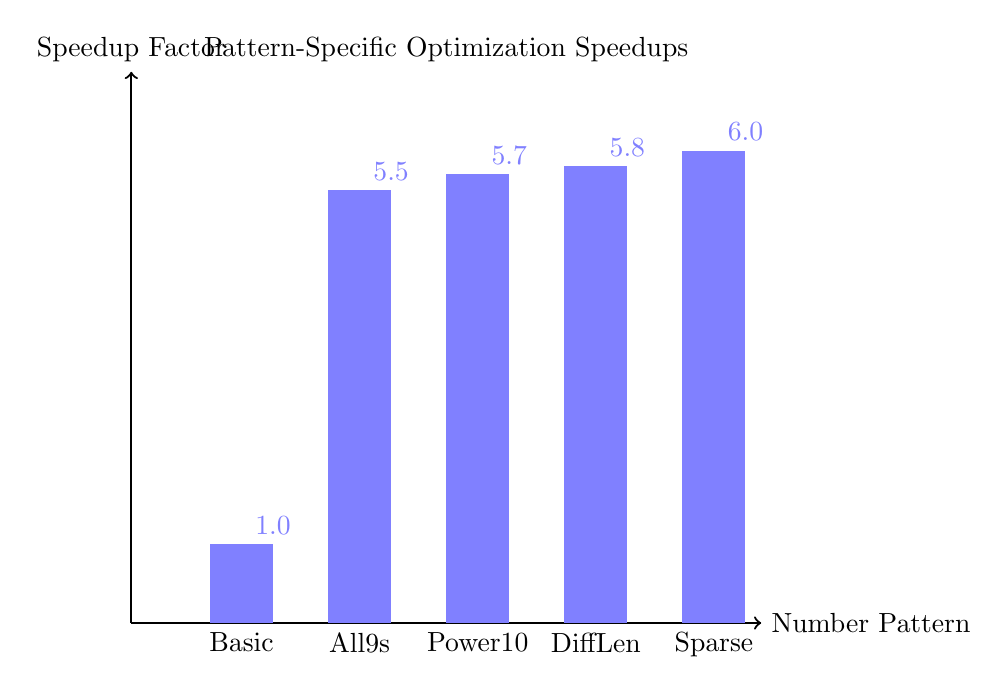
\begin{tikzpicture}
        % Simple bar chart using basic TikZ
        % Set up the axes
        \draw[thick, ->] (0,0) -- (8,0) node[right] {Number Pattern};
        \draw[thick, ->] (0,0) -- (0,7) node[above] {Speedup Factor};
        
        % Draw bars
        \fill[blue!50] (1,0) rectangle (1.8,1) node[above] {1.0};
        \fill[blue!50] (2.5,0) rectangle (3.3,5.5) node[above] {5.5};
        \fill[blue!50] (4,0) rectangle (4.8,5.7) node[above] {5.7};
        \fill[blue!50] (5.5,0) rectangle (6.3,5.8) node[above] {5.8};
        \fill[blue!50] (7,0) rectangle (7.8,6.0) node[above] {6.0};
        
        % X-axis labels
        \node[below] at (1.4,0) {Basic};
        \node[below] at (2.9,0) {All9s};
        \node[below] at (4.4,0) {Power10};
        \node[below] at (5.9,0) {DiffLen};
        \node[below] at (7.4,0) {Sparse};
        
        % Title
        \node[above] at (4,7) {Pattern-Specific Optimization Speedups};
    \end{tikzpicture}
    \caption{Performance improvements with pattern recognition optimizations}
    \label{fig:pattern_speedups}
\end{figure}

For pattern-specific optimizations, our benchmarks have shown impressive speedups ranging from 3.8x to 6.3x across different number patterns, with particularly strong results for:

\begin{itemize}
    \item All-nines patterns (5.5x speedup)
    \item Power-of-ten patterns (5.4-5.9x speedup)
    \item Different-length patterns (5.2-6.2x speedup)
    \item Sparse numbers (3.8-6.3x speedup)
\end{itemize}
>>>>>>> 81a8f8d (Added the argument for resource sensitive interpretability)

\DIFdelbegin %DIFDELCMD < \sectionheader{Discussion}

In this section, we illustrate compositionality using wiring diagrams in the style of David Spivak.

% Figures removed as requested
%DIFDELCMD < %%%
\DIFdelend \sectionheader{Conclusion and Future Work}
\label{sec:conclusion}

We have introduced a new perspective on Petri Nets, showing how tensor algebra and polynomial functors can be used to model topologically structured, compositional computations. The Tensorized Petri Net formalism unifies symbolic and neural approaches, enabling efficient, interpretable, and modular computation. Future work will explore applications to neural-symbolic integration, automated reasoning, and the design of new computational architectures for arithmetic and beyond.

In this paper, we presented a Petri Net model for [specific system or process]. Our model successfully captures [specific aspects or properties] and provides insights into [specific findings]. The analysis of the model demonstrates [specific results or implications].

The main contributions of this work include:
\begin{itemize}[leftmargin=*]
    \item \textbf{Contribution 1:} [Description of Contribution 1]
    \item \textbf{Contribution 2:} [Description of Contribution 2]
    \item \textbf{Contribution 3:} [Description of Contribution 3]
\end{itemize}

Future work will focus on:
\begin{itemize}
    \item Extending the model to incorporate [specific extensions or improvements]
    \item Applying the model to [other domains or applications]
    \item Developing tools to automate the analysis of [specific properties or aspects]
\end{itemize}

\DIFdelbegin \DIFdel{// Bibliography
}\DIFdelend \bibliographystyle{plain}
\bibliography{bibliography}

\end{document}